\chapter{Технологическая часть}

В данной части приведены средства реализации, реализации алгоритмов и функциональные тесты.

\section{Средства реализации}

Для реализации последовательного и параллельного алгоритмов проверки связности графа использовался язык программирования C++ (стандарт C++17)~\cite{cpp_standard}. 
Параллельная версия реализована средствами стандартной библиотеки: \texttt{std::thread} для запуска потоков, \texttt{std::mutex} и \texttt{$std::condition_variable$} для синхронизации доступа к общей очереди, а также \texttt{std::atomic} для атомарной отметки посещённых вершин~\cite{cpp_standard}.

Сборка выполнялась компилятором \texttt{g++} из состава gcc~\cite{gcc}.

Для получения временных замеров в исследовании использована функция \texttt{clock()} из заголовочного файла \texttt{<ctime>}~\cite{cpp_standard}.

\section{Схемы алгоритмов}

Схемы последовательной и параллельной реализаций проверки связности представлены на рисунках~\ref{fig:bfs-seq} и~\ref{fig:bfs-par}.

Оценка вычислительной сложности обхода в ширину (BFS):
\begin{equation}
T_{\mathrm{BFS}} = O\!\left(|V| + |E|\right),
\label{eq:bfs-complexity}
\end{equation}
где $|V|$ --- число вершин, $|E|$ --- число рёбер.


\section{Демонстрация работы программы}

На рисунке~\ref{fig:prog} представлена демонстрация работы программы, выполняющей проверку связности графа параллельным алгоритмом BFS.

\begin{figure}[H]
    \centering
    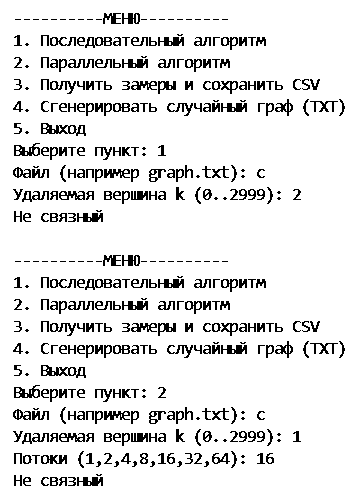
\includegraphics[width=0.6\textwidth]{images/prog.png}
    \caption{Параллельная версия алгоритма BFS (проверка связности)}
    \label{fig:prog}
\end{figure}

\section{Функциональные тесты}



Для проверки корректности работы последовательного и параллельного алгоритмов проверки связности графа были разработаны функциональные тесты.
Тестирование выполнялось для различных классов графов: пустой граф, граф из одной вершины, связный граф, несвязный граф, а также графы, содержащие изолированные вершины.
Результаты тестирования представлены в таблице~\ref{tab:func-tests-format}.

В таблице граф задаётся списком смежности в виде
$u \rightarrow \{v_1, v_2, \dots\}$, где $u$ --- номер вершины, а $v_i$ --- номера вершин, в которые существуют рёбра из $u$.
Ожидаемый результат и получаемый результат представляются как булево значение:
\texttt{true} --- граф связен (все вершины достижимы из стартовой вершины $0$),
\texttt{false} --- граф несвязен.

\begin{table}[H]
\centering
\caption{Пример представления результатов функциональных тестов алгоритмов проверки связности}
\label{tab:func-tests-format}
\renewcommand{\arraystretch}{1.15}
\small
\begin{tabular}{|p{2.8cm}|p{4.4cm}|p{4.4cm}|p{4.4cm}|}
\hline
\textbf{Граф} & \textbf{Ожидаемый результат} & \textbf{Последовательный алгоритм} & \textbf{Параллельный алгоритм} \\ \hline

\begin{minipage}[t]{\linewidth}
\textbf{Тест 1:} $n=0$ \\
(пустой граф)
\end{minipage}
&
\begin{minipage}[t]{\linewidth}
\textbf{Ожидаем:} \texttt{true} \\
Пустой граф считается связным.
\end{minipage}
&
\begin{minipage}[t]{\linewidth}
\textbf{\texttt{conn\_seq}:} \texttt{true} \\
Условие $g.n==0$.
\end{minipage}
&
\begin{minipage}[t]{\linewidth}
\textbf{\texttt{conn\_par}:} \texttt{true} \\
Условие $g.n==0$.
\end{minipage}
\\ \hline

\begin{minipage}[t]{\linewidth}
\textbf{Тест 2:} $n=4$ \\
$0 \rightarrow 1$ \\
$1 \rightarrow 0,2$ \\
$2 \rightarrow 1,3$ \\
$3 \rightarrow 2$
\end{minipage}
&
\begin{minipage}[t]{\linewidth}
\textbf{Ожидаем:} \texttt{true} \\
Все вершины достижимы из 0.
\end{minipage}
&
\begin{minipage}[t]{\linewidth}
\textbf{\texttt{conn\_seq}:} \texttt{true} \\
Посещены: $0,1,2,3$.
\end{minipage}
&
\begin{minipage}[t]{\linewidth}
\textbf{\texttt{conn\_par}:} \texttt{true} \\
Посещены: $0,1,2,3$.
\end{minipage}
\\ \hline

\begin{minipage}[t]{\linewidth}
\textbf{Тест 3:} $n=5$ \\
$0 \rightarrow 1$ \\
$1 \rightarrow 0,2$ \\
$2 \rightarrow 1$ \\
$3 \rightarrow 4$ \\
$4 \rightarrow 3$
\end{minipage}
&
\begin{minipage}[t]{\linewidth}
\textbf{Ожидаем:} \texttt{false} \\
Вершины $3$ и $4$ \\
не достижимы из 0.
\end{minipage}
&
\begin{minipage}[t]{\linewidth}
\textbf{\texttt{conn\_seq}:} \texttt{false} \\
Посещены: $0,1,2$. \\
не посетили: $3,4$.
\end{minipage}
&
\begin{minipage}[t]{\linewidth}
\textbf{\texttt{conn\_par}:} \texttt{false} \\
Посещены: $0,1,2$. \\
не посетили: $3,4$.
\end{minipage}
\\ \hline

\end{tabular}
\end{table}



По результатам функционального тестирования установлено, что последовательный и параллельный алгоритмы корректно определяют связность графа на рассмотренных наборах входных данных: результаты, полученные при выполнении \texttt{conn\_seq} и \texttt{conn\_par}, совпадают с ожидаемыми значениями.


\section*{Вывод}

В технологической части выбраны средства разработки и описана реализация последовательного и параллельного алгоритмов проверки связности графа.
Также приведены схемы алгоритмов и указаны используемые средства измерения времени выполнения.


\clearpage